\documentclass[12pt, titlepage]{article}

\usepackage{fullpage}
\usepackage[round]{natbib}
\usepackage{multirow}
\usepackage{booktabs}
\usepackage{tabularx}
\usepackage{graphicx}
\usepackage{float}
\usepackage{hyperref}
\hypersetup{
    colorlinks,
    citecolor=blue,
    filecolor=black,
    linkcolor=red,
    urlcolor=blue
}
\usepackage{graphicx}
\graphicspath{ {./images/} }
\usepackage{caption}
\usepackage{enumitem}
\input{../../Comments}
%% Common Parts

\newcommand{\progname}{Chess Connect} % PUT YOUR PROGRAM NAME HERE
\newcommand{\authname}{Team \#4,
\\ Alexander Van Kralingen
\\ Arshdeep Aujla
\\ Jonathan Cels
\\ Joshua Chapman
\\ Rupinder Nagra} % AUTHOR NAMES without MacIDs 

\usepackage{hyperref}
    \hypersetup{colorlinks=true, linkcolor=blue, citecolor=blue, filecolor=blue,
                urlcolor=blue, unicode=false}
    \urlstyle{same}

\newcommand{\projectoverview}{

The Chess Connect project allows two users to play a game of chess on a physical board with the information being transmitted to an online web application over Bluetooth.
Currently, there is no way for players to seamlessly switch between playing on a physical board and playing online, but Chess Connect intends to change this by creating a central platform that will provide flexibility and remove barriers for new players looking to learn the game.

}

\newcounter{acnum}
\newcommand{\actheacnum}{AC\theacnum}
\newcommand{\acref}[1]{AC\ref{#1}}

\newcounter{ucnum}
\newcommand{\uctheucnum}{UC\theucnum}
\newcommand{\uref}[1]{UC\ref{#1}}

\newcounter{mnum}
\newcommand{\mthemnum}{M\themnum}
\newcommand{\mref}[1]{M\ref{#1}}

\begin{document}

\title{System Design for \progname} 
\author{\authname}
\date{\today}

\maketitle

\pagenumbering{roman}

\section{Revision History}

\begin{tabularx}{\textwidth}{p{3cm}p{2cm}X}
\toprule {\bf Date} & {\bf Version} & {\bf Notes}\\
\midrule
2023-01-11 & Arshdeep Aujla & Added Introduction, Purpose, User Interface, Other Considered Designs \\
2023-01-17 & Arshdeep Aujla & Added Design of Hardware \\
\bottomrule
\end{tabularx}

\newpage

\section{Reference Material}

This section records information for easy reference.

\subsection{Abbreviations and Acronyms}

\renewcommand{\arraystretch}{1.2}
\begin{tabular}{l l} 
  \toprule		
  \textbf{symbol} & \textbf{description}\\
  \midrule 
  \progname & Explanation of program name\\
  \wss{...} & \wss{...}\\
  \bottomrule
\end{tabular}\\

\newpage

\tableofcontents

\newpage

\listoftables

\listoffigures

\newpage

\pagenumbering{arabic}

\section{Introduction}
This document outlines the system design portion of this project's design documentation. Design documentation 
is intended to separate the project into modular components to increase the project's understandability and reusability. \\
Other useful documents for this project are the following:
\begin{itemize}
  \item SRS
  \item HA
  \item VnV
\end{itemize}

\section{Purpose}
The purpose of this document is to outline a detailed system design. The system design includes system variables, user interfaces, a timeline for completion, and designs of many 
different components such as hardware, electrical components, and communication protocols. This document also includes references to an intensive list of the project's
mechanical and electrical components and a reflection in the appendix. \\
Other documents relating to design are the following:
\begin{itemize}
  \item Software Architecture Document
  \item Detailed Design Document
\end{itemize}
\section{Scope}

\wss{Include a figure that show the System Context (showing the boundary between
your system and the environment around it.)}

\section{Project Overview}

\subsection{Normal Behaviour}

\subsection{Undesired Event Handling}

\wss{How you will approach undesired events}

\subsection{Component Diagram}

\subsection{Connection Between Requirements and Design} \label{SecConnection}

\wss{The intention of this section is to document decisions that are made
  ``between'' the requirements and the design.  To satisfy some requirements,
  design decisions need to be made.  Rather than make these decisions implicit,
  they are explicitly recorded here.  For instance, if a program has security
  requirements, a specific design decision may be made to satisfy those
  requirements with a password.}

\section{System Variables}

\wss{Include this section for Mechatronics projects}

\subsection{Monitored Variables}

\subsection{Controlled Variables}

\subsection{Constants Variables}

\section{User Interfaces}

\subsection{Hardware Interface}
The user will interact with two main components of the hardware.
\begin{itemize}
  \item Magnetic chess pieces
  \item Physical chess board containing sensors
\end{itemize}
They will interact with the chess pieces and chess board as they would in a normal chess game. The chess board reflects a standard chess board, with 
LEDs in the center of each square. They would move the chess pieces on the board and remove them in according to the rules of chess. If the device
is set to beginner mode, the LEDs will light up in according to which available moves are available for that chess piece. They would interact with the LEDs
by using them as a guide for potential moves to make.

\subsection{Software Interface}
The users will interact with the software component of this device through a web application. They would need a device with an internet connection and and internet browser
to view the application. The user will interact with this interface by visual viewing the chess board status in real time including a visualization of the chess piece locations.
They will also be able to turn on and off beginner mode in this interface through clicking an interactive button in the web application. 

\section{Design of Hardware}

Each square on the chessboard will contain a Hall sensor and a green LED. The LEDs are to indicate where a piece can possibly go, depending on which mode the user is in. For example, 
if the user is in a beginner’s mode and picks up the White King, then the LEDs surrounding all the squares where the King is picked up from will light up telling the user that the 
King can be placed on any of those squares. The logic for which LEDs light up depend on a few things:
\begin{itemize}
  \item The type of piece. Different LEDs would light up for King, Queen etc.
  \item If any of the user’s own color piece is placed on a square, that LED would not light up as you cannot place two pieces on the same square. However, if an opponent’s piece is 
  placed on a square, that LED may light up provided it is a valid move depending on the type of piece the user is making the move with.
  \item Any square further away from a square where user’s own piece is present, will not light up as the pieces cannot jump a piece unless it is a Knight.
\end{itemize}
  Let us see the working of the LEDs considering the example on a 5x5 grid as shown in the figure below. ‘1-5’ are the rows and ‘A-E’ are the columns. ‘a-e’ are the twenty-five different LEDs corresponding to 
  each square. The green background squares will indicate the LED to be ON for that square in the grid.

  \begin{figure}[h]
    \centering
    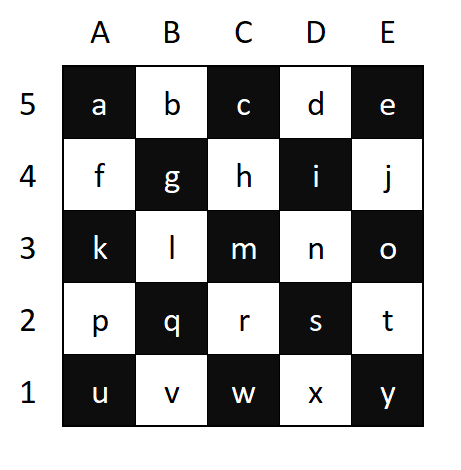
\includegraphics[width=0.5\textwidth]{line2}
    \caption{5x5 Grid}
  \end{figure}

  \begin{itemize}
    \item Case 1: King present in the middle of a 5x5 grid chessboard. The King can move only one square in any direction – up, down, to the sides, and diagonally.

    \begin{minipage}{\linewidth}
      \centering
      
\includegraphics[width=0.5\textwidth]{king}
      \captionof{figure}{Potential moves for the King}
  \end{minipage}

  The LEDs g,h,i,l,n,q,r,s will light up for the potential moves provided those squares are empty or an opponent’s piece is placed on those squares.

    \item Case 2: Queen present in the middle of a 5x5 grid chessboard. The Queen can move multiple squares in any one direction - forward, backward, sideways and 
    diagonally as far as possible as long as she does not move through any of her own pieces.

    \begin{minipage}{\linewidth}
      \centering
      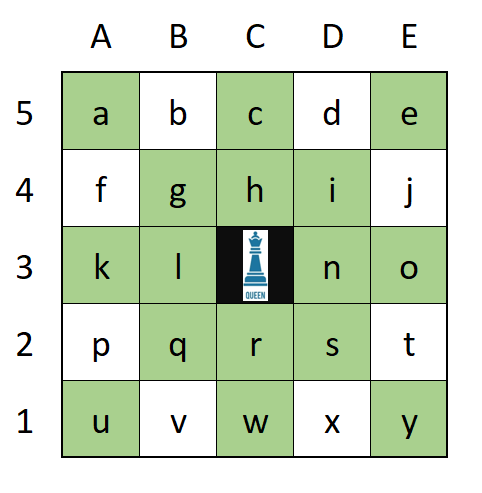
\includegraphics[width=0.5\textwidth]{queen}
      \captionof{figure}{Potential moves for the Queen}
  \end{minipage}

  The LEDs a,c,e,g,h,i,k,l,n,o,q,r,s,u,w,y will light up for the potential moves provided those squares are empty or an opponent’s piece is placed on those squares.

    \item Case 3: Bishop present in the middle of a 5x5 grid chessboard. The Bishop can move multiple squares but only diagonally. Each bishop starts on one color (light or dark) 
    and must always stay on that color. 

    \begin{minipage}{\linewidth}
      \centering
      
\includegraphics[width=0.5\textwidth]{bishop}
      \captionof{figure}{Potential moves for the Bishop}
  \end{minipage}

  The LEDs a,e,g,i,q,s,u,y will light up for the potential moves provided those squares are empty or an opponent’s piece is placed on those squares.

    \item Case 4: Knight present in the middle of a 5x5 grid chessboard. The Knight can move two squares in one direction, and then one more move at a 90-degree angle in either 
    direction, just like the shape of an “L”. 

    \begin{minipage}{\linewidth}
      \centering
      
\includegraphics[width=0.5\textwidth]{knight}
      \captionof{figure}{Potential moves for the Knight}
  \end{minipage}

  The LEDs b,d,f,j,p,t,v,x will light up for the potential moves provided those squares are empty or an opponent’s piece is placed on those squares. Knight is the only chess 
  piece that can skip over a piece and be placed even if it is immediately surrounded by a user’s own piece. For example, if there is user’s own pieces present at the 
  squares B2, B3 and B4, the user can still place the Knight at A2, A4, B1 or B6 by skipping over the other pieces.

    \item Case 5: Rook present in the middle of a 5x5 grid chessboard. The Rook can move multiple squares but only forward, backward or to the sides. 
  
    \begin{minipage}{\linewidth}
      \centering
      
\includegraphics[width=0.5\textwidth]{rook}
      \captionof{figure}{Potential moves for the Rook}
  \end{minipage}

  The LEDs c,h,k,l,n,o,r,w will light up for the potential moves provided those squares are empty or an opponent’s piece is placed on those squares.

    \item Case 6: Pawn present in the middle of a 5x5 grid chessboard. Pawns are unusual because they move and capture in different ways: they move forward but capture 
    diagonally. Pawns can only move forward one square at a time, except for their very first move where they can move forward two squares.

    \begin{minipage}{\linewidth}
      \centering
      
\includegraphics[width=0.5\textwidth]{pawn}
      \captionof{figure}{Potential moves for the Pawn}
  \end{minipage}

  The LEDs c,g,h,i will light up for the potential moves provided those squares are empty or an opponent’s piece is placed on those squares. For pawn, the LED ‘c’ only 
  lights up if it is the first time a pawn is making a move. After a pawn has been moved once, it can never move two squares at once. Also, a pawn can move diagonally, 
  only if there is an opponent’s piece is present on those squares. Otherwise, it can only move in the forward direction. For example, the LED ‘g’ or ‘i’ will only light 
  up if there is an opponent’s piece present on them. 

  \end{itemize}
  


\subsection*{Truth Table for LEDs}

Based on the assumptions above, the Truth Table for the LEDs 'a-y' would as shown in the figure below. 
The digit '0' means LED is OFF and '1' means LED is ON.

\begin{figure}[h]
  \centering
  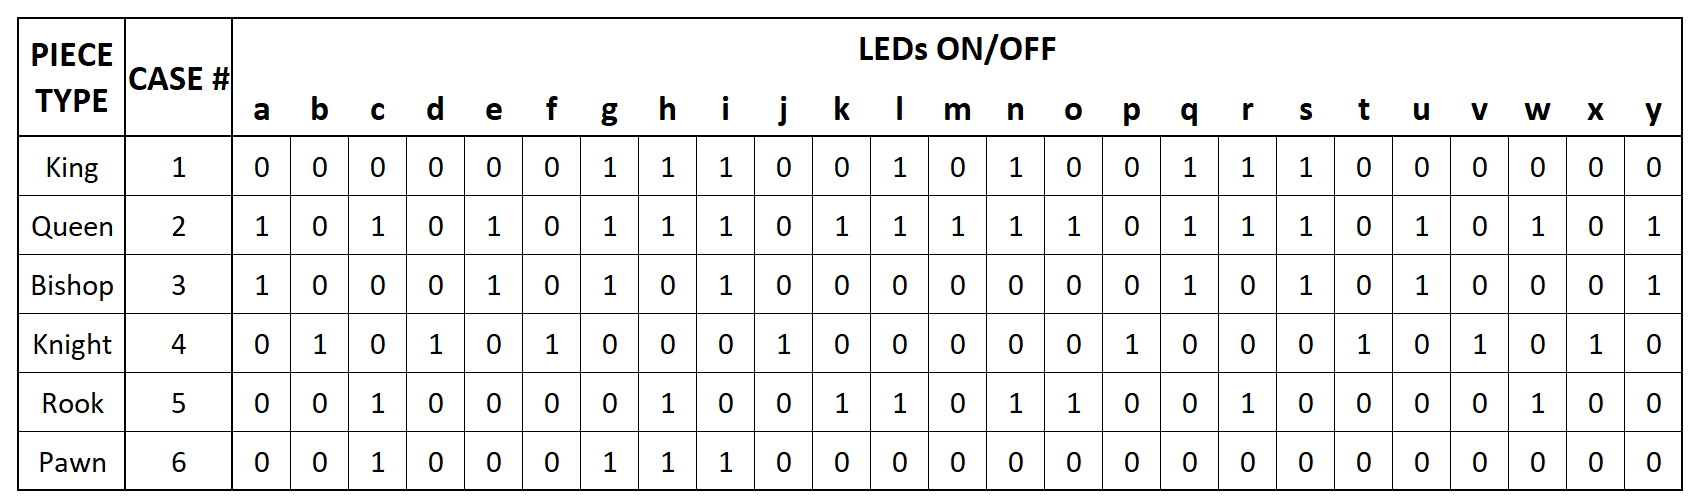
\includegraphics[width=1\textwidth]{truth_table}
  \caption{Truth Table}
\end{figure}

\subsection{Components Acquired}
Please refer to Appendix B for a detailed list of acquired mechanical components.

\section{Design of Electrical Components}
\subsection{Components Acquired}
Please refer to Appendix C for a detailed list of acquired electrical components.

\wss{Most relevant for mechatronics projects}
\wss{Show what will be acquired}
\wss{Show what will be built, with detail on fabrication and materials}
\wss{Include appendices as appropriate, possibly with sketches, drawings,
circuit diagrams, etc}

\section{Design of Communication Protocols}

\wss{If appropriate}

\section{Timeline}

\wss{Schedule of tasks and who is responsible}

% \bibliographystyle {plainnat}
% \bibliography{../../../refs/References}

\newpage{}

\appendix

\section{Interface}

\wss{Include additional information related to the appearance of, and
interaction with, the user interface}

\section{Mechanical Hardware}
\begin{itemize}
  \item Arduino Mega
\end{itemize}

\section{Electrical Components}
\begin{itemize}
  \item 64 LEDs
  \item 64 1000ohm resistors
  \item 64 HALL sensors
  \item 64 1mF capacitors
  \item 3 breadboards
  \item 300 pieces of wire
\end{itemize}

\section{Communication Protocols}

\section{Reflection}

\subsection*{Project Limitations}

\subsection*{Other Considered Designs}
One problem that we had to overcome in our design is that there are not enough input and output pins in one microcontroller for all of the components.
One solution we considered was having multiple microcontrollers for this project to ensure there is one input pin for each input sensor and one output pin for each output.
This design would be beneficial in the way of simplicity of code. The tradeoff would be the complexity in coordinating the communication between multiple microcontrollers and the 
web application. A second option to solve this problem is to use multiplexing to reduce the number of input and output pins needed for a large number of components. 
This option requires more complex code, but only requires one microcontroller device. We chose to implement the multiplexing option because it only used one device which saves money,
as well as eliminates the need to coordinate between multiple microcontrollers. 

The information in this section will be used to evaluate the team members on the
graduate attribute of Problem Analysis and Design.  Please answer the following questions:

\begin{enumerate}
  \item What are the limitations of your solution?  Put another way, given
  unlimited resources, what could you do to make the project better? (LO\_ProbSolutions)
  \item Give a brief overview of other design solutions you considered.  What
  are the benefits and tradeoffs of those other designs compared with the chosen
  design?  From all the potential options, why did you select documented design?
  (LO\_Explores)
\end{enumerate}

\end{document}